\subsection{Descripción del problema.}

\vspace*{0.3cm}

\textbf{Introducción} \newline
En esta época en que el tiempo es muy valioso(''el tiempo es oro''), y no estaría bueno perderlo. Y los alumno del pabellón  cero+infinito no son la excepción. \newline
El edificio fue diseñado con una cantidad de pasillos que podría ser excesivo, y esto traería problemas a los alumno, docentes y comunidad exactas. \newline
 A este problema lo podemos modelar como un grafo ponderado(con pesos en las aristas), donde cada eje es un pasillo y su peso es la longitud del pasillo. Los vértices serian las intersecciones entre pasillos o un extremo dónde termina el dicho pasillo.
En las figuras de abajo vemos un pasillo, el pabellón cero+infinito, y también una muy posible distribución de pasillos de dicho pabellón.  
\begin{figure}[H]
  \begin{center}
      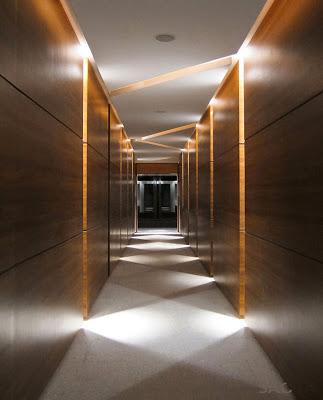
\includegraphics[scale=0.40]{imagenes/pasillo1.jpeg}
      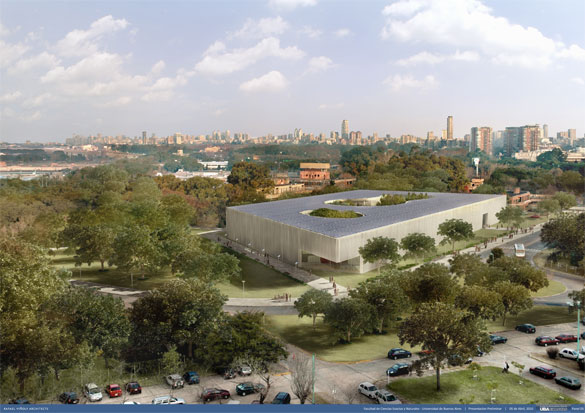
\includegraphics[scale=0.40]{imagenes/cero+infinito1.jpg}
      \caption{Pasillo moderno, pabellón Cero+infinito}
  \end{center}
  \begin{center}    
      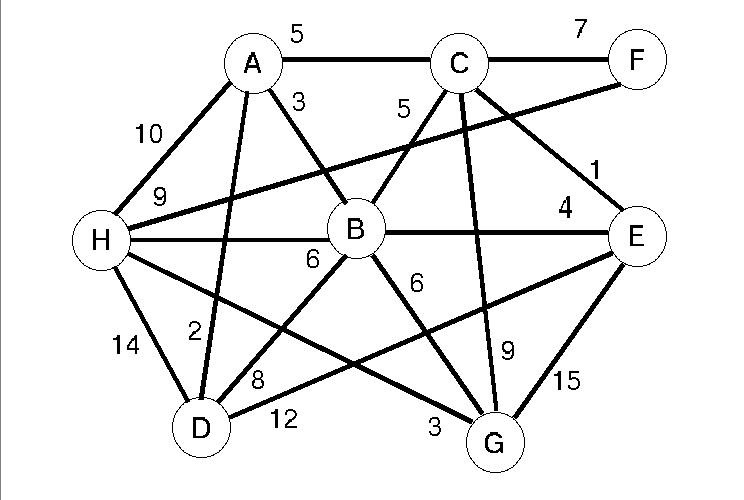
\includegraphics[scale=0.30]{imagenes/grafoPasillo.jpg}
       \caption{Ejemplo de distribución de pasillos del pabellón}
  \end{center}
%  \caption{ejemplo}
\end{figure}

\textbf{Problema} \newline
El decano y el Director del Departamento de Computación, se reunieron para charlar sobre el problema de la mala distribución de los pasillos.
El problemas es que se podrían generar ciclos en el grafo que representa los pasillos, y esto desorientaría a muchos alumnos (peor los alumnos ciclarían infinitamente). Por consiguiente se tomaron medidas para remediar este problema. Se decidió clausurar pasillos de modo tal que queden un grafo sin ciclos. \newline   
Para clausurar hay que tener en cuenta lo siguiente :

\begin{itemize}  
	\item Los pasillos mas largos son más costosos de clausurar.
	\item Debemos devolver la mínima suma de longitudes de pasillos que deben ser clausurados(podría ser ninguno).
	\item La solución la debemos devolver con complejidad $O(M*log(M))$, donde  $M = \# ConjuntoDePasillos$ (cantidad de aristas).
	\item Como precondición tenemos que el grafo es conexo.
\end{itemize}
Como vemos este problema es un caso típico de optimización(en este caso minimización). Acá se quiere minimizar la suma posible de longitudes de pasillos que se quieren clausurar. \newline

En las siguientes lineas vamos a tener conjuntos de 3-uplas que representan las aristas, donde primer y segundo componente son los nodos de incidencia, la tercer componente es el peso de la arista. \newline
  
\textbf{Ejemplos de input y output: } \newline
En las siguientes lineas vamos a tener conjuntos de 3-uplas que representan las aristas, donde primer y segundo componente son los nodos de incidencia, la tercer componente es el peso de la arista.\newline
Ejemplo 1:

\begin{center}
\begin{tikzpicture}[node distance   = 2 cm]
  %\useasboundingbox (-1,-1) rectangle (11,11); 
  \tikzset{VertexStyle/.style = {shape          = circle,
                                 ball color     = orange,
                                 text           = black,
                                 inner sep      = 2pt,
                                 outer sep      = 0pt,
                                 minimum size   = 24 pt}}
  \tikzset{EdgeStyle/.style   = {thick,
                                 double          = orange,
                                 double distance = 1pt}}
  \tikzset{LabelStyle/.style =   {draw,
                                  fill           = yellow,
                                  text           = red}}
     \node[VertexStyle](A){A};
     \node[VertexStyle,right=of A](B){B};
     \node[VertexStyle,right=of B](C){C};
     \tikzset{EdgeStyle/.append style = {bend left}}
     \draw[EdgeStyle](A) to node[LabelStyle]{3} (B);
     \draw[EdgeStyle](B) to node[LabelStyle]{3} (C);
     \draw[EdgeStyle](C) to node[LabelStyle]{3} (A);
  \end{tikzpicture}

\end{center}

\begin{itemize}  
	\item Entrada:  $\{(A,B,3),(B,C,3),(C,A,3) \}$
%	\item Salida: 3, podemos borrar solamente una arista cualquiera (en el dibujo borramos la arista (A,C,3)) para eliminar el ciclo.
\end{itemize}


\begin{center}
\begin{tikzpicture}[node distance   = 2 cm]
  %\useasboundingbox (-1,-1) rectangle (11,11); 
  \tikzset{VertexStyle/.style = {shape          = circle,
                                 ball color     = orange,
                                 text           = black,
                                 inner sep      = 2pt,
                                 outer sep      = 0pt,
                                 minimum size   = 24 pt}}
  \tikzset{EdgeStyle/.style   = {thick,
                                 double          = orange,
                                 double distance = 1pt}}
  \tikzset{LabelStyle/.style =   {draw,
                                  fill           = yellow,
                                  text           = red}}
     \node[VertexStyle](A){A};
     \node[VertexStyle,right=of A](B){B};
     \node[VertexStyle,right=of B](C){C};
     \tikzset{EdgeStyle/.append style = {bend left}}
     \draw[EdgeStyle](A) to node[LabelStyle]{3} (B);
     \draw[EdgeStyle](B) to node[LabelStyle]{3} (C);
  \end{tikzpicture}
\end{center}


\begin{itemize}  
%	\item Entrada:  $\{(A,B,3),(B,C,3),(C,A,3) \}$
	\item Salida: 3, podemos borrar solamente una arista cualquiera (en el dibujo borramos la arista (A,C,3)) para eliminar el ciclo.
\end{itemize}

Ejemplo 2: \newline

\begin{center}
\begin{tikzpicture}[node distance   = 2 cm]
%  \useasboundingbox (-1,-1) rectangle (11,11); 
  \tikzset{VertexStyle/.style = {shape          = circle,
                                 ball color     = orange,
                                 text           = black,
                                 inner sep      = 2pt,
                                 outer sep      = 0pt,
                                 minimum size   = 12 pt}}
  \tikzset{EdgeStyle/.style   = {thick,
                                 double          = orange,
                                 double distance = 2 pt}}
  \tikzset{LabelStyle/.style =   {draw,
                                  fill           = yellow,
                                  text           = red}}
     \node[VertexStyle](A){A};
     \node[VertexStyle,right=of A](B){B};
     \node[VertexStyle,right=of B](C){C};
%     \node[VertexStyle,right=of C](E)(E);
     \node[VertexStyle,above= 4 cm of A](D){D};     
     \node[VertexStyle,above= 4 cm of C](E){E};     

     \draw[EdgeStyle](A) to node[LabelStyle]{8} (B) ;
     \tikzset{EdgeStyle/.append style = {bend left}}
     \draw[EdgeStyle](C) to node[LabelStyle]{10} (D);
     \draw[EdgeStyle](A) to node[LabelStyle]{70} (E);
%     \draw[EdgeStyle](B) to node[LabelStyle]{3} (A);
     \draw[EdgeStyle](A) to node[LabelStyle]{63} (D);
     \draw[EdgeStyle](B) to node[LabelStyle]{53} (C);
     \draw[EdgeStyle](B) to node[LabelStyle]{54} (E);

     \draw[EdgeStyle](E) to node[LabelStyle]{12} (C);
     \draw[EdgeStyle](D) to node[LabelStyle]{22} (E);
  \end{tikzpicture}
\end{center}

\begin{itemize}  
	\item Entrada:  $\{(A,B,8),(A,E,70),(A,D,63),(B,C,53),(B,E,54),(C,D,10),(C,E,12),(D,E,22)\}$
\end{itemize}


\begin{center}
\begin{tikzpicture}[node distance   = 2 cm]
%  \useasboundingbox (-1,-1) rectangle (11,11); 
  \tikzset{VertexStyle/.style = {shape          = circle,
                                 ball color     = orange,
                                 text           = black,
                                 inner sep      = 2pt,
                                 outer sep      = 0pt,
                                 minimum size   = 12 pt}}
  \tikzset{EdgeStyle/.style   = {thick,
                                 double          = orange,
                                 double distance = 2 pt}}
  \tikzset{LabelStyle/.style =   {draw,
                                  fill           = yellow,
                                  text           = red}}
     \node[VertexStyle](A){A};
     \node[VertexStyle,right=of A](B){B};
     \node[VertexStyle,right=of B](C){C};
     \node[VertexStyle,above= 4 cm of A](D){D};     
     \node[VertexStyle,above= 4 cm of C](E){E};     
     \tikzset{EdgeStyle/.append style = {bend left}}
     \draw[EdgeStyle](A) to node[LabelStyle]{70} (E);
     \draw[EdgeStyle](A) to node[LabelStyle]{63} (D);
     \draw[EdgeStyle](B) to node[LabelStyle]{53} (C);
     \draw[EdgeStyle](B) to node[LabelStyle]{54} (E);
  \end{tikzpicture}
\end{center}

\begin{itemize}  
	\item Salida: 52, que es la suma de los pesos mínimos de las aristas que debo borrar (52 = 8+10+12+22), para sacar los ciclos de este grafo.
\end{itemize}

Observar que en los dos ejemplos anteriores encontramos el árbol generador máximo.
%\begin{itemize}
	%\item Entrada:  $\{(A,B,3),(B,C,3),(C,A,3) /}$ 
	%\item Salida: 3
%\end{itemize}	


%\begin{center}
%\begin{tikzpicture}[node distance   = 4 cm]
%  \useasboundingbox (-1,-1) rectangle (11,11); 
%  \tikzset{VertexStyle/.style = {shape          = circle,
%                                 ball color     = orange,
%                                 text           = black,
%                                 inner sep      = 2pt,
%                                 outer sep      = 0pt,
%                                 minimum size   = 24 pt}}
%  \tikzset{EdgeStyle/.style   = {thick,
%                                 double          = orange,
%                                 double distance = 1pt}}
%  \tikzset{LabelStyle/.style =   {draw,
%                                  fill           = yellow,
%                                  text           = red}}
%     \node[VertexStyle](A){A};
%     \node[VertexStyle,right=of A](B){B};
%     \node[VertexStyle,right=of B](C){C};
%     \node[VertexStyle,above= 8 cm of B](D){D};     
%     \draw[EdgeStyle](B) to node[LabelStyle]{1} (D) ;
%     \tikzset{EdgeStyle/.append style = {bend left}}
%     \draw[EdgeStyle](A) to node[LabelStyle]{2} (B);
%     \draw[EdgeStyle](B) to node[LabelStyle]{3} (A);
 %    \draw[EdgeStyle](B) to node[LabelStyle]{4} (C);
%     \draw[EdgeStyle](C) to node[LabelStyle]{5} (B);
%     \draw[EdgeStyle](A) to node[LabelStyle]{6} (D);
%     \draw[EdgeStyle](D) to node[LabelStyle]{7} (C);

%  \end{tikzpicture}
%\end{center}
%\end{document}

%\begin{figure}[htb]
%  \begin{center}
%      \includegraphics[scale=0.25]{imagenes/ejemplo.jpg}
%  \end{center}
%  \caption{ejemplo}
%\end{figure}


\subsection{Desarrollo de la idea y pseudocódigo.}

\vspace*{0.3cm}


Vamos a crear un árbol generador máximo del grafo de pasillos, para así quedarnos con los ejes más chicos que forman un ciclo. La suma de estos ejes es el costo mínimo a pagar para eliminar los ciclos en el grafo.
Para que este problema nos de en orden O($m*log(m)$), siendo m la cantidad de pasillos, utilizaremos la representación en lista de adyacencia del grafo de pasillos. Para generar el árbol generador máximo usaremos un algoritmo muy parecido de Kruskal junto con UnionFind, para que nos de en complejidad pedida. La diferencia entre Kruskal y nuestro algoritmo es que este en vez de agarrar primero las aristas más chicas, tomará las aristas más grande, formado el árbol generador máximo.

\textbf{pseudocodigo} %\newline 

\begin{codebox}
\Procname{$\proc{solve}(int \ n, vector<Aristas> \& portales)	$}
	\li \Comment inicializo $conj$, como un conj vacio y $peso$ en cero
	\li $Ordenar(portales)$	
	\li \Comment Ordeno de mayor a menor segun la longitud del pasillo
	\li \For $i \gets 0$ \To $portales.size$ \Do
	\li		\If generaCiclos($portales[i]$)
	\li			\Then $peso $=$ peso $+$ portales[i].longitud$
	\li 				\Else agregar($conj, portales[i]$) 
			\End
		\End
	\li \Return $peso$
\end{codebox}


\subsection{Justificación de la resolución y demostración de correctitud.}

\vspace*{0.3cm}

%\textbf{completar!}
Ahora probaremos que el algoritmo prepuesto resuelve el problema. Lo que se quiere es eliminar los ciclos con el menor costo. El eliminar los ciclos nos deja un árbol generador del grafo de pasillos, ya que queda un grafo acíclico y conexo. Si el grafo que queda no es conexo significa que habríamos sacado una arista que era el único camino posible entre, por lo menos, un par de nodos, lo que dice que esa arista no era parte de un ciclo. Entonces una solución con esa arista nos daría un costo menor. \newline 
Ahora, como queremos un árbol generador que deje afuera la aristas menos pesadas, para conseguir un costo mínimo, tenemos que generar un árbol que contenga las aristas mas pesadas de los ciclo del grafo, para que queden fuera de este la más livianas. Esto lo hacemos de la misma manera en que el algoritmo de Kruskal genera un AGM, en cada paso agregamos la arista con el peso máximo que no genera ciclos, por lo que nos queda un árbol generador máximo. Por lo tanto, las aristas que quedaron fuera de ese árbol son las aristas más livianas que, al agregarlas, forman un ciclo en el grafo, así que sumadas dan el costo mínimo para eliminar los ciclos.

\subsection{Análisis de complejidad.}

\vspace*{0.3cm}

%\textbf{completar!}
La complejidad de este algoritmo es O($m*log(m)$) siendo m la cantidad de pasillos, ya que esto es lo que tarda realizar el Kruskal modificado.\newline
 El Kruskal modificado tiene complejidad O($m*log(m)$) ya que su  operación más costosa, y la primera en realizarse, es ordenar las aristas y esto lo hace en O($m*log(m)$) ya que sort de \verb-C++- tarda O($n*log(n)$)(según la biblioteca standar de \verb-C++-), siendo n la cantidad de elementos en la lista. Como sort ordena de menor a mayor, lo siguiente en hacerse es usar la instrucción reverse de \verb-C++- que tiene O$\left(\displaystyle\frac{n}{2}\right)$(según biblioteca estándar de \verb-C++-) y la vuelta los valores del vector. Después realizamos la operación de crear un UnionFind para los vértices que tiene O($v$), siendo v la cantidad de vértices, pero $m>=v-1$, por ser un grafo conexo, por lo que es O($m$). Por último, realizamos un for donde todas las operaciones dentro de él son O($1$) o son, Union, para que los dos vértices de la arista agregada a el árbol estén en el mismo conjunto, o isSameSet, para verificar que los extremos de la arista no estén en el mismo conjunto ya que si es así, entonces al agregarla se generaría un ciclo. Entonces, como vimos en clase, si hay una secuencia de m operaciones de makeSet, findSet, unionSet, estas se vuelve orden constante, lo que deja a todos las operaciones del for en O($m$)\newline
 Este algoritmo, con cantidad de vértices(v) y aristas(m) constantes, no tiene un mejor o peor caso, ya que se tienen que recorrer siempre todas las aristas. Se puede hablar de un mejor o peor caso según la cantidad de vértices del grafo, ya que teniendo una cantidad v de vértices uno puede tener más o menos aristas. Entonces podemos hablar de un peor caso el grafo es completo, ya que es la máxima cantidad$\left(\displaystyle\frac{v*(v-1)}{2}\right)$ de aristas que podría tener dado un v. Y de un mejor caso cuando el grafo ya sea un árbol($v-1$), es decir no tiene ciclos, ya que es la menor cantidad de aristas que puede tener un grafo conexo dado un v. Suponiendo que sort de c verifica si la lista esta ordenada y que esto lo hace en orden lineal podemos hacer que nuestro mejor caso deje las aristas ordenadas de menor a mayor, esto generaría que su complejidad sea O($m$) en vez de O($m*log(m)$).

\subsection{Experimentación y gráficos.}

Par las instancias de toma de tiempos del problema 3 lo que hacemos es, si queremos un mejor caso, desde 1 hasta v, siendo v la cantidad de vértices, creamos una arista de el vértice actual al siguiente con peso igual al vértice, para así generar un árbol, y que las aristas estén ordenadas por su peso. Si lo que buscamos es un peor caso, desde 1 hasta v, creamos aristas que van desde el vértice actual hasta todos los siguientes con un peso random, así generamos un grafo completo. Esto se puede realizar por $instanciasEj3.cpp$, pero al utilizarlo nos dimos cuanta que las instancias podían ser muy grandes y pesadas. Por lo cual decidimos hacer que el mismo $TP2EJ3.cpp$ genere cada instancia y tome los tiempos, esto se hace pasando como parámetro un 2.\newline
Para tomar los tiempos corremos 100 veces cada instancia y tomamos el promedio de los resultados que estén entre el promedio más la desvío estándar y el promedio menos el desvío estándar. Este desvío lo calculamos realizando la raíz cuadrada de la varianza, que se puede calcular restándole a cada uno de los tiempos el promedio, elevándolos al cuadrado y después se saca el promedio de todos esos.
\newline\newline
En los siguientes gráficos tenemos los resultados obtenidos...

\begin{figure}[H]
  \begin{center}
      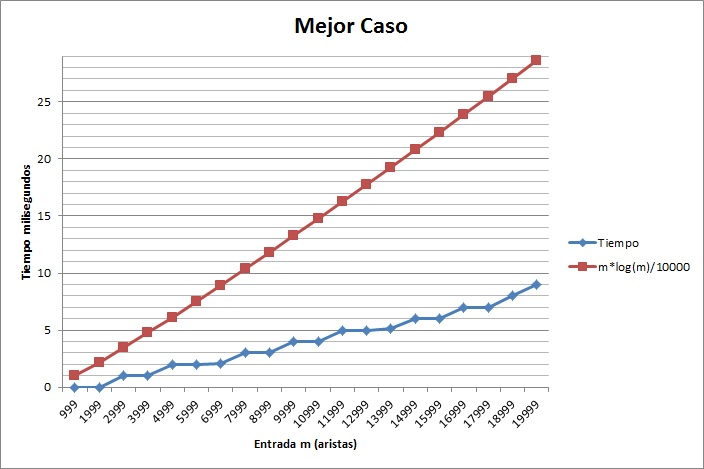
\includegraphics[scale=0.70]{../MejorCasoEj3.jpg}
  \end{center}
 \end{figure}

Este gráfico muestra como el mejor caso de nuestro algoritmo esta siempre acotado por la curva $m*log(m)$. También muestra que a medida que hay más cantidad de vértices la curva con nuestros tiempos se aleja de la curva $m*log(m)$ lo que permite suponer con mayor certeza que el sort de c tarda menos si las aristas ya están ordenadas. Este gráfico apoya nuestra demostración de complejidad, aunque no lo comprueba, porque este caso siempre va a tener mejor tiempo que los otros.

\begin{figure}[H]
  \begin{center}
      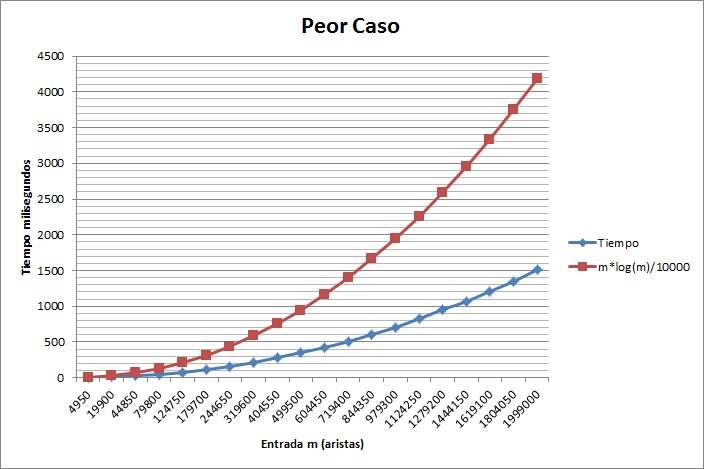
\includegraphics[scale=0.70]{../PeorCasoEj3.jpg}
  \end{center}
 \end{figure}

Este segundo gráfico permite corroborar con más certeza que el anterior la cota en nuestra complejidad, ya que muestra como una curva $m*log(m)$ acota todos los tiempos tomados para el peor caso y, además, se puede observar que nuestros tiempos forman una curva similar a la de $m*log(m)$. También se puede ver como estas dos curvas se van alejando a medida que aumenta la cantidad de vértices.

\subsection{Validación}

Para validar el algoritmo, utilizamos casos de test, los cuales son una expansión de los test de la cátedra, para los cuales conocemos cual es la salida. Las instancia para validar se encuentran en $Tp2Ej3.in$ y las salidas correspondientes a esas instancias se encuentran en $Tp2Ej3.out$. Corriendo $TP2EJ3.cpp$ con los parámetros 1 y $Tp2Ej3.in$ se obtienen los resultados de nuestro algoritmo para esas instancias, estas se guardan en el archivo $TP2Ej3nuestro.out$. Se pueden comparar ambas archivos corriendo $testCorrectitud.cpp$ pasando como parámetro las dos salidas.